\documentclass[11pt, oneside]{article}
\usepackage[a4paper,bindingoffset=0.2in,%
            left=1in,right=1in,top=1in,bottom=1in,%
            footskip=.25in]{geometry}
\usepackage{graphicx}
\usepackage{enumerate}
\usepackage{url}
\usepackage{hyperref}
\usepackage{pbox}
\usepackage{CJKutf8}
\usepackage{mathtools}
\usepackage{microtype}
\usepackage[htt]{hyphenat}
\renewcommand{\vec}[1]{\mathbf{#1}}


\begin{document}
\title{Semester Project: Gaussian Mixture Model}
\author{Xiyou Zhou, 13307130189 \\ Computer Science and Technology}
\maketitle

\section{Gaussian Mixture Model with EM Algorithm}

I start with plotting with 3 different Gaussian Distributions.

One is at $\mu = (0, 0), \Sigma = \begin{bmatrix} 
50 & 20 \\
30 & 40 
\end{bmatrix}$ with 2500 points, one is at $\mu = (50, 40), \Sigma = \begin{bmatrix} 
400 & 500 \\
200 & 400 
\end{bmatrix}$ with 3000 points, and the last one is at $\mu = (-10, 40), \Sigma = \begin{bmatrix} 
100 & 20 \\
60 & 40 
\end{bmatrix}$ with 4500 points.

The initial parameters are set with a KMeans result of 3 kernels. After 30 epochs, the distribution of three clusters changed from 30\%, 25\% and 45\% to 25\%, 30\% and 45\%. The kernel location changed from (4.30, 0.99), (54.54, 46.57), (-9.77, 40.01) to (0.10, -0.07), (49.79, 39.93), (-9.77, 40.05).

\section{Gaussian Mixture Model with Gibbs Sampling}
Not finished. Will implement later in the summer.

\section{Analysis}

Complex models generally leads to more accurate results and more data can help generate more accurate estimation. EM Algorithm and Gibbs Sampling both can be applied to latent parameter estimation. However, EM Algorithm always maximizes the result of certain likelihood function while Gibbs Sampling can be constructed from Monte-Carlo Markov Chain and its convergence is also guaranteed by MCMC.

EM as a maximization/maximization method, Gibbs as a variation of Generalized EM. Instead of
maximizing at each of these two steps(E, M), Gibbs algorithm use the conditional distributions to sample from them.


\begin{thebibliography}{9}

\bibitem{NYUGMMEM}
New York University: Mixture Models EM algorithm, Lecture 21
\\\texttt{http://cs.nyu.edu/\~{}dsontag/courses/ml12/slides/lecture21.pdf}

\bibitem{gibbs}
C19: Lecture 4: A Gibbs Sampler for Gaussian Mixture Models\\
\texttt{http://www.robots.ox.ac.uk/\~{}fwood/teaching/C19\_hilary\_2013\_2014/gmm.pdf}

\bibitem{cmu}
Gibbs and Metropolis sampling (MCMC methods)\\
\texttt{http://www.cs.cmu.edu/\~{}tom/10-702/GibbsAndMCMCsampling.pdf}

\end{thebibliography}

\section{Appendix}
\begin{figure}[h]
\centering
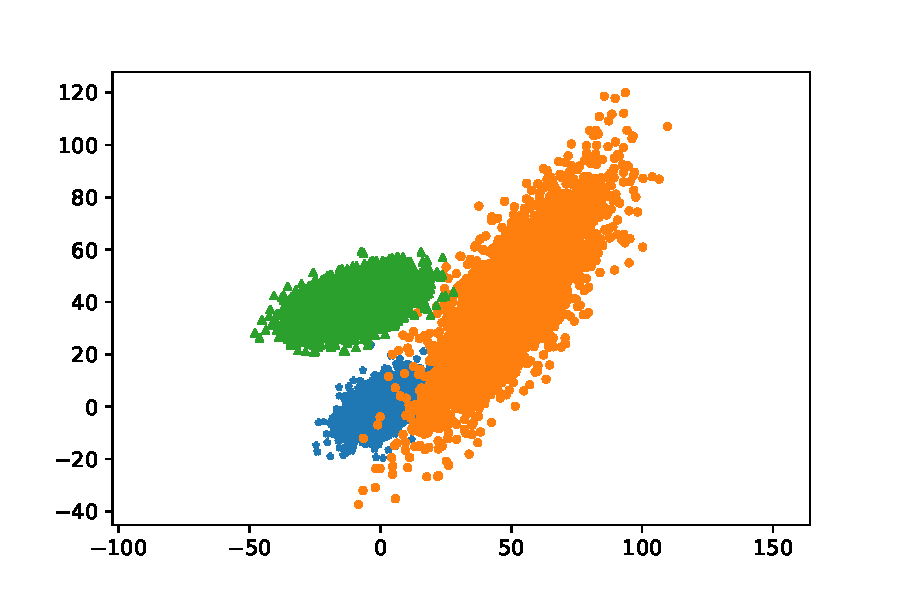
\includegraphics{origin.pdf}
\caption{Plot of original distribution of all points}
\centering
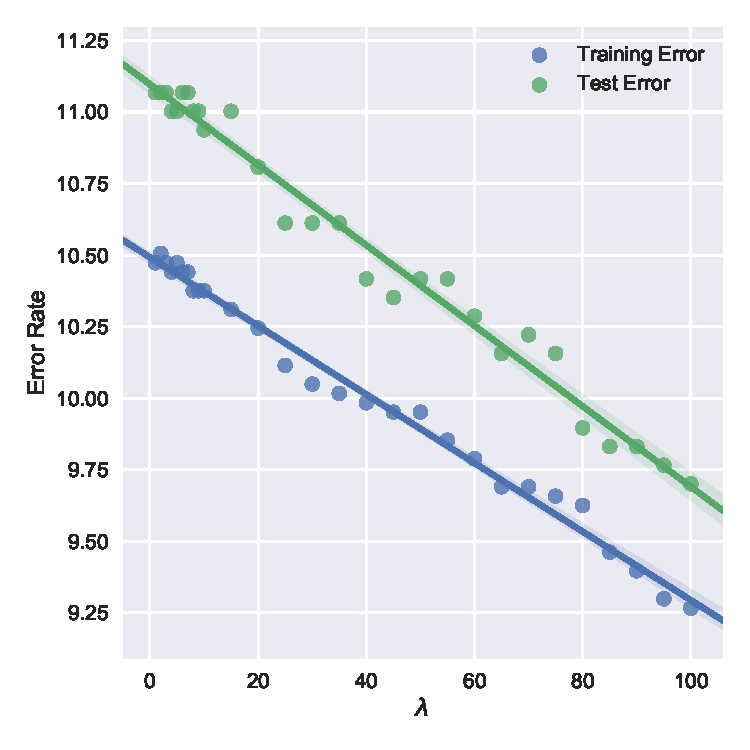
\includegraphics{foo.pdf}
\caption{Plot of EM Algorithm fit result after 30 epochs}
\end{figure}

\end{document}